% Lecture Template for ME3050-001-002-Tristan Hill - Spring 2020
% Dynamics Modeling and Controls
% Time Response - Lecture 2

% I am finally converting my stuff to BEAMER

% Document settings

%\documentclass{beamer}                  % for presentation ?
\documentclass[handout]{beamer}  % for handout ?
\usepackage{beamerthemesplit}
\usepackage{amsmath}
\usepackage{listings}
\usepackage{multicol}

\beamertemplateballitem

\definecolor{TTUpurple}{rgb}{0.3098, 0.1607, 0.5176} % TTU Purple (primary)
\definecolor{TTUgold}{rgb}{1.0000, 0.8666, 0.0000} % TTU Gold (primary)

\setbeamercolor{palette primary}{bg=TTUpurple,fg=TTUgold}
\setbeamercolor{palette secondary}{bg=black,fg=TTUgold}
\setbeamercolor{palette tertiary}{bg=black,fg=TTUpurple}
\setbeamercolor{palette quaternary}{bg=TTUgold,fg=black}
\setbeamercolor{structure}{fg=TTUpurple} % itemize, enumerate, etc
\setbeamercolor{section in toc}{fg=TTUpurple} % TOC sections

%\usefonttheme{professionalfonts}

\newcommand{\LNUM}{2\hspace{2mm}} % Lecture Number 

\newcommand{\vspcc}{\vspace{6mm}\\ } 
\newcommand{\vspc}{\vspace{3mm}\\ } 
\newcommand{\hspc}{\hspace{5mm} } 

\newcommand{\Lagr}{\mathcal{L}} % lagrangian

\newcommand{\secondtitle}{Free Response of Second Order Systems}% second line of the title of this presentation , aka the topic of this lecture

\title{Time Response - Lecture \LNUM}
\author{ME3050 - Dynamics Modeling and Controls} % original formatting from Mike Renfro, September 21, 2004

\date{April 03, 2020}

\begin{document}

\lstset{language=MATLAB,basicstyle=\ttfamily\small,showstringspaces=false}

% Title page
\frame{\titlepage \center\textbf{\secondtitle}\vspcc}


% Section 0: Outline
\frame{

\large \textbf{Lecture \LNUM - \secondtitle} \vspc

 \begin{itemize}

	\item Second Order Systems with No Damping\vspc % Section 1

	\item Second Order Systems with Damping\vspc        % Section 2

	\item The Damping Ratio \vspc   %Section 3

\end{itemize}

}

% Section 1: Second Order System with No Damping
\section{ Second Order System with No Damping}

\subsection{Mass Spring Model}
\frame{
\frametitle{Mass Spring Model}

\large Consider the mass-spring system without damping.\vspc

			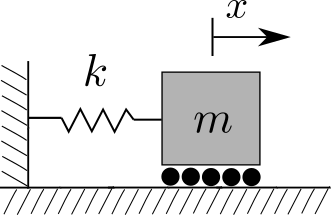
\includegraphics[scale=.5]{mass_spring_01.png} \vspc

\large The EOM is:\vspc

	\scalebox{1.0}{$m\ddot{x} +kx=0$\hspc with} \vspc
	\scalebox{1.0}{$ x(t=0)=x_0$, \hspc and\hspc$v(t=0)=v_0$}\vspc

}


\subsection{Solution with Laplace Transforms Method} 

\frame{
\frametitle{Solution with Laplace Transforms Method}

\large Solve for $x(t)$ with a method of your choice. \vspace{40mm}\\


\scalebox{1.0}{$x(t)=\frac{v_0}{\omega_n}sin(\omega_nt)+x_0cos(w_nt) $\hspc with\hspc $\omega_n=\sqrt{\frac{k}{m}}$} \vspc
}

\subsection{Phase Shift} 

\frame{
\frametitle{Phase Shift}

\large The solution is commonly written as a single oscillating term with a {\bf phase shift} $\phi$.\vspc

	\scalebox{1.0}{$x(t)=\frac{v_0}{\omega_n}sin(\omega_nt)+x_0cos(w_nt) $\hspc with\hspc $\omega_n=\sqrt{\frac{k}{m}}$} \vspc

\large Is equivalent to: \vspc

	\scalebox{1.0}{$x(t)=Acos(\omega_nt-\phi)$\hspc$A=\sqrt{x_0^2+[\frac{v_0}{\omega_n}]^2}$\hspc$\phi=tan^{-1}(\frac{v_0}{x_0\omega_n})$} \vspc

\large Sine could be used instead.\vspc

\scalebox{1.0}{$x(t)=Asin(\omega_nt+\phi)$\hspc$A=\sqrt{x_0^2+[\frac{v_0}{\omega_n}]^2}$\hspc$\phi=tan^{-1}(\frac{x(0)\omega_n}{v_0})$} \\

}

\subsection{Sketch of Free Response} 

\frame{
\frametitle{Sketch of Free Response}

\large Sketch the {\bf free} response in the time domain.  \vspc

\scalebox{1.0}{$x(t)=\frac{v_0}{\omega_n}sin(\omega_nt)+x_0cos(w_nt) $ }  \vspc
\scalebox{1.0}{$=Acos(\omega_nt-\phi)$\hspc$with$\hspc$\phi=tan^{-1}(\frac{v_0}{x_0\omega_n})$}  \vspc

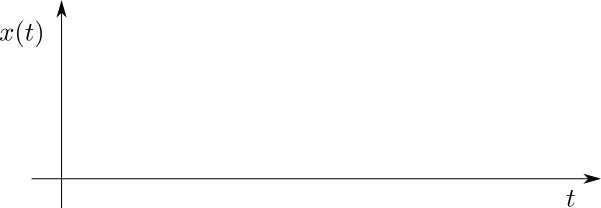
\includegraphics[scale=0.5]{lecture2_fig2.png} \\

\large Is this a stable system? What does the phase shift $\phi$ represent? \\

}

% Section 2: Second Order Systems with Damping
\section{Second Order Systems with Damping}
\subsection{Mass-Spring-Damper Model}

\frame{
\frametitle{Second Order System with Damping}

\large Now, consider the mass-spring system with damping present.\vspc

	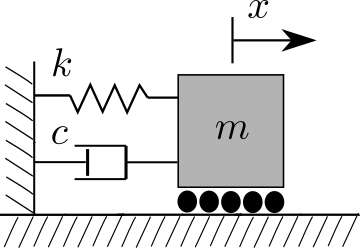
\includegraphics[scale=.4]{mass_spring_02.png} \hspc 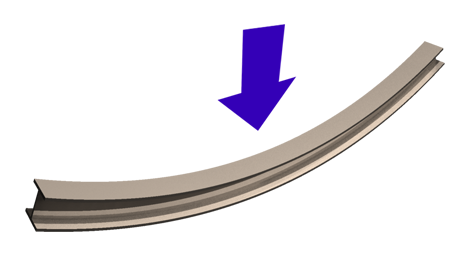
\includegraphics[scale=.20]{beam_bending_01.png} 

\large The EOM is:\vspc

	\scalebox{1.0}{$m\ddot{x} +c\dot{x}+kx=0$\hspc with} \vspc
	\scalebox{1.0}{$ x(t=0)=x_0$, \hspc and\hspc$v(t=0)=v_0$}\vspc

}


\subsection{Solution with Laplace Transforms Method} 

\frame{
\frametitle{Solution with Trial Solution Method}

The trial solution method is used to derive the response equation in terms of the system variables and parameters. \vspc

%\large The affects of damping can be seen in the reponse equations.  \vspc

	\scalebox{1.0}{$m\ddot{x} +c\dot{x}+kx=0$ $ \implies$  $(mr^2+cr+k)Ae^{rt}=0$} \vspc

\large You can see the {\it characteristic equation} becomes: \vspc
	\scalebox{1.0}{$(mr^2+cr+k)=0$}   \vspc

\large Solve for the roots. In system dynamics they are called $s_{1,2}$  \vspc

	\scalebox{1.0}{$r_{1,2}=s_{1,2}=\frac{-c\pm\sqrt{c^2-4mk}}{2m}=-\frac{c}{2m}\pm\sqrt{(\frac{c}{2m})^2-\frac{k}{m}}$}   \vspc

}


\frame{
\frametitle{The Roots of the System}

\large The roots of the system determine the behavior.  \vspc

\scalebox{1.0}{$s_{1,2}=\frac{-c\pm\sqrt{c^2-4mk}}{2m}$}\vspc

The {\bf discriminant} $c^2-4mk$ drives the {\it case} in the trial solution method. \vspc

\begin{itemize}
\item IF \underline{\hspace{20mm}} $\implies$Case 1: Distinct and Real \vspace{1mm}\\
\item IF \underline{\hspace{20mm}} $\implies$Case 2: Repeated and Real \vspace{1mm}\\
\item IF \underline{\hspace{20mm}} $\implies$Case 3: Complex Conjugate Pair \vspc
\end{itemize}
}


\subsection{Damping Cases and the Critical Damping Value}
\frame{
\frametitle{Damping Cases and the Critical Damping Value}

\large In a system with known mass and spring constant, the damping value determines the behavior. The damping value that causes the {\it discriminant} to equal zero (case 2) is the {\bf critical damping value}.  \vspc

\scalebox{1}{$c^2-4mk = 0 \implies c=\sqrt{4mk}=2\sqrt{mk}$} \vspcc

\scalebox{1.}{$c_{critical}=2\sqrt{mk}$} \vspc




}

\subsection{The Damping Ratio}
\frame{

\frametitle{The Damping Ratio}

\large The damping ratio $\zeta$ is the ratio of damping c to the critical damping value $c_{critical}$. \vspace{2mm}\\

\scalebox{1.0}{$\zeta=\frac{c}{c_{critical}}=\frac{c}{2\sqrt{mk}}$} \vspace{2mm}\\

\large Re-write the roots with this new quantity. \vspace{2mm}\\

\scalebox{1.0}{$s_{1,2}=-\zeta\omega_n\pm\omega_n\sqrt{\zeta^2-1}=-\zeta\omega_n\pm j\omega_n\sqrt{1-\zeta^2}$}  \vspace{2mm}\\

\large We define a new quantity, {\bf damped natural frequency}.  \vspace{2mm}\\
	
\scalebox{1.0}{$\omega_d=\omega_n\sqrt{1-\zeta^2}$}  \vspace{2mm}\\

\large Now re-write the roots again in terms of $\zeta$ and $\omega_d$.  \vspace{2mm}\\

\scalebox{1.0}{$s_{1,2}=\zeta\omega_n\pm j\omega_d$}  \vspace{2mm}\\
 
}



\frame{
\frametitle{Forms of the Response Equations}

\large The behavior of the system depends on the damping ratio.  \vspcc


\renewcommand{\arraystretch}{2}
\begin{tabular}{|c|c|c|c|}
Case 1&\scalebox{1.0}{$c>2\sqrt{mk}$ }&{\bf Overdamped}&\scalebox{1}{$\zeta>1$} \\
Case 2&\scalebox{1.0}{$c=2\sqrt{mk}=c_{critical}$ }&{\bf Critically Damped}&\scalebox{1}{$\zeta=1$}\\
Case 3&\scalebox{1.0}{$c<2\sqrt{mk}$ }&{\bf Underdamped}&\scalebox{1}{$\zeta<1$} \\
\end{tabular}

}


\frame{
\frametitle{The Overdamped Case}

The roots are real and distinct and the system {\it does not} oscillate. \vspc

\large \underline{Overdamped}\hspc $c>2\sqrt{mk} \hspc \implies\hspc \zeta>1$ \hspc \vspcc

\scalebox{1}{$s_{1,2}=-\zeta\pm\omega_n\sqrt{\zeta^2-1}$}\vspc

\scalebox{1}{$x(t)=C_1e^{(-\zeta\omega_n+\omega_n\sqrt{\zeta^2-1}\hspace{1mm})t}+C_2e^{(-\zeta\omega_n-\omega_n\sqrt{\zeta^2-1}\hspace{1mm})t}$}\vspc

\scalebox{1}{$x(t)=e^{-\zeta\omega_n}\{C_1e^{\omega_n\sqrt{\zeta^2-1}t}+C_2e^{\omega_n\sqrt{\zeta^2-1}t}\}$}\vspc
\scalebox{1}{$C_1=\frac{-v_0+(-\zeta+\sqrt{\zeta^2-1})\omega_nx_0}{2\omega_n\sqrt{\zeta^2-1}}$}\hspc
\scalebox{1}{$C_2=\frac{-v_0+(\zeta+\sqrt{\zeta^2-1})\omega_nx_0}{2\omega_n\sqrt{\zeta^2-1}}$} \vspc


}

\frame{
\frametitle{The Critically Damped Case}

The roots are real and repeated and the system {\it does not} oscillate. \vspcc

\large \underline{Critically Damped}\hspc $c=2\sqrt{mk} \hspc \implies\hspc \zeta=1$ \hspc \vspcc

\scalebox{1}{$s_{1,2}=\frac{-c}{2m}=\zeta\omega_n=-\omega_n$}\vspc

\scalebox{1}{$x(t)=C_1e^{-\omega_nt}+C_2te^{-\omega_nt}$}\vspc

\scalebox{1}{$\dot{x}=-\omega_nC_1e^{-\omega_nt}+C_2t(-\omega_ne^{-\omega_nt})+e^{-\omega_nt}(C_2)$} \vspc

\scalebox{1}{$x(t=0)=x_0\implies C_1=x_0$}\vspc

\scalebox{1}{$v(t=0)=v_0\Rightarrow v_0=-\omega_nC_1+0+(1)C_2 \implies C_2=v_0+\omega_nx_0$}\vspc

}

\frame{
\frametitle{The Underdamped Case}

The roots are a complex conjugate pair and the system oscillates. \vspcc

\large \underline{Underdamped}\hspc $c<2\sqrt{mk} \hspc \implies\hspc \zeta<1$ \hspc \vspcc

\scalebox{1}{$s_{1,2}=-\zeta\omega_n\pm j\omega_d$}\vspc

\scalebox{1}{$x(t)=C_1e^{(\zeta\omega_n+j\omega_d)t}+C_2e^{(\zeta\omega_n-j\omega_d)t}$}\vspc

\scalebox{1}{$x(t)=e^{-\zeta\omega_nt}\{Acos(\omega_dt)+Bsin(\omega_dt)\}$}\vspc

Use the initial position to solve for the first unknown. \vspc

\scalebox{1}{$x(t=0)=x_0=(1)(A(1)+B(0))\implies A=x_0$}\vspc
}


\frame{
\frametitle{The Underdamped Case}

Take the derivative and solve for the second unknown. \vspc

\scalebox{1}{$x(t)=e^{-\zeta\omega_nt}\{Acos(\omega_dt)+Bsin(\omega_dt)\}$}\vspc

\scalebox{1}{$\dot{x}(t)=e^{-\zeta\omega_nt}(-\omega_dAsin(\omega_dt))+Acos(\omega_dt)(-\zeta\omega_ne^{-\zeta\omega_nt})$}\vspc

\scalebox{1}{$+e^{-\zeta\omega_nt}(\omega_dBcos(\omega_dt))+Bsin(\omega_dt)e^{-\zeta\omega_nt}$}\vspc

\scalebox{1}{$\dot{x}(t=0)=A(1)(-\zeta\omega_n(1))+(1)\omega_dB(1)\implies B=\frac{v_0+\zeta\omega_nx_0}{\omega_d}$}\vspc

Finally we get to the reponse equation. \vspc

\scalebox{1}{$x(t)=e^{-\zeta\omega_nt}\{x_0cos(\omega_dt)+\frac{v_0+\zeta\omega_nx_0}{\omega_d}sin(\omega_dt)\}$}

}


\frame{
\frametitle{Response of the Three Different Cases}

\large Each of the three cases behaves in a {\it characteristic} way.\vspcc
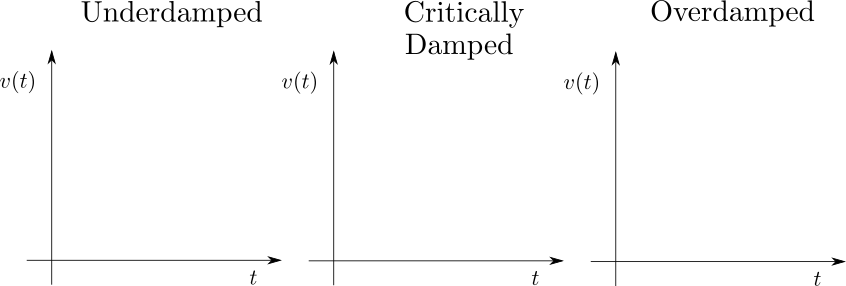
\includegraphics[scale=0.5]{lecture2_fig3.png} 

}

\frame{
\frametitle{Affects of Damping Ratio and Damped Natural Frequency}

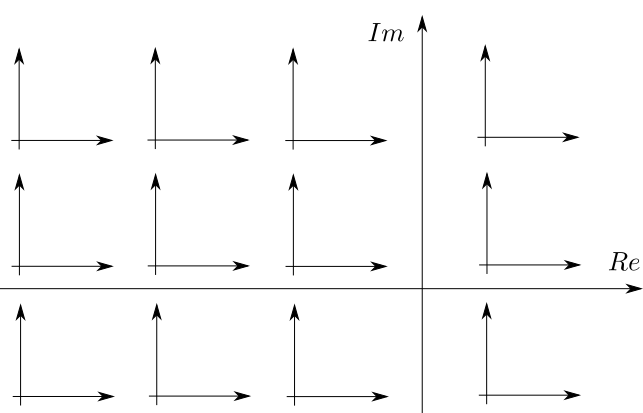
\includegraphics[scale=0.60]{lecture2_fig4.png} 

}

%\frame{
%
%\frametitle{Graph the affects of damping ratio}
%
%}

%% Section 3: Forced Response of a Second Order Model % I think this section goes in the next lecture... 
%\section{ Forced Response of a Second Order Model}
%
%\frame{
%
%\frametitle{Second Order System Subject to Step Input}
%
%\large Now, consider the mass-spring system with damping present subject to step input. This models instantly turning on the input force $f(t)$.\vspc
%
%\begin{multicols}{2}
%
%	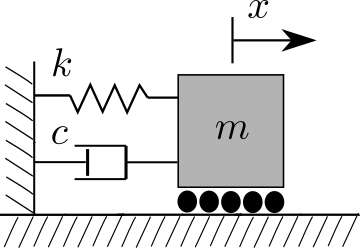
\includegraphics[scale=.4]{mass_spring_02.png} \hspc  
%
%	\[f(t) = \begin{cases} 
%	      0 & t < 0 \\
%	      F & t\geq 0 \\
%	   \end{cases}
%	\]\\
%
%\end{multicols}
%
%\large The EOM is:\vspc
%
%	\scalebox{1.0}{$m\ddot{x} +c\dot{x}+kx=f(t)$\hspace{3mm}with\hspace{3mm}$x(t=0)=x_0$\hspace{3mm}and\hspace{3mm}$v(t=0)=v_0$}\vspc
%
%}


% references is not a section for now, for looks and it would be a waste of space
\frame{

\frametitle{References}

\begin{itemize}
	\item System Dynamics, Palm III, Third Edition - Section 8.2 - Response of Second Order Systems - pg. 484
\end{itemize}

}
\end{document}









 